\documentclass[a4paper,12pt,twoside=false]{scrartcl}

\usepackage[T1]{fontenc}        %Umlaute und Akzente
%\usepackage[latin1]{inputenc}
\usepackage[utf8x]{inputenc}    %UTF-8
\usepackage[ngerman]{babel}     %neue Rechtschreibung & richtige Silbentrennung
%\usepackage{nomencl}           %Abkürzungen definieren
%\usepackage{pxfonts} 			% griechisches Alphabet
\usepackage{amsmath,amsthm,amsfonts,amssymb} %mathematische Bibliotheken
%\usepackage{scrpage}
%\usepackage{csquotes}          % zusätzliche Optionen zum Zitieren
%\usepackage{url}            %URLs hinzufügen
\usepackage{xcolor}
\usepackage{colortbl}
\usepackage[boxed]{algorithm}
\usepackage{algorithmic}
\usepackage[small]{caption}      %kleine Untertitel
\usepackage{setspace}  
\usepackage{relsize}          %Zeilenabstand ändern
%\usepackage{ulem}               %erweiterte Optionen zum Unterstreichen
\usepackage{multicol}           % Text in Spalten ermöglichen
\usepackage{enumerate}           %?
\usepackage[pdftex]{graphicx}    %Grafiken ermöglichen
\usepackage{pdfpages}
\usepackage{tikz}
\usepackage{longtable}
\usepackage{multirow}
\definecolor{darkgreen}{cmyk}{0.9,0.0,0.8,0.0}
\definecolor{lightgreen}{cmyk}{0.9,0.0,0.3,0.0}
\definecolor{mauve}{RGB}{224 176 255}
\definecolor{mauveL}{RGB}{160 160 255}

\usetikzlibrary{arrows,calc} 
\usepackage[pdftex]{hyperref}    %Hyperlinks ermöglichen
\definecolor{linkcolor}{rgb}{0, 0, 0.7}
\hypersetup{
  pdfstartview = FitH,
  breaklinks = true,
  colorlinks = true,
  bookmarksopen = true,
  linkcolor = linkcolor,
  anchorcolor = linkcolor,
  citecolor = linkcolor,
  filecolor = linkcolor,
  menucolor = linkcolor,
  urlcolor = linkcolor
}


\setlength{\parindent}{0em}     %Kein Einrücken von Absätzen

%\pagestyle{plain}
%\pagestyle{scrheadings}
%\renewcommand\sectionmark[1]{\markright{#1}}
%\renewcommand\chaptermark[1]{\markboth{#1}{}}
%%\ohead{\headmark}
%\headsep=1.5cm


\newtheoremstyle{dfn_style}           % name
  {10pt}            % Space above
  {10pt}            % Space below
  {}              % Body font
  {}              % Indent amount 1
  {\bfseries}            % Theorem head font
  {}              % Punctuation after theorem head
  {.5em}            % Space after theorem head 2
  {\thmname{#1}\thmnumber{ #2}.\thmnote{ #3}}    % Theorem head spec (can be
                                                  %left empty, meaning ‘normal’)


\newtheoremstyle{satz_style}        % name
  {10pt}        % Space above
  {10pt}        % Space below
  {\itshape}    % Body font
  {}            % Indent amount 1
  {\bfseries}   % Theorem head font
  {}            % Punctuation after theorem head
  {.5em}        % Space after theorem head (must not be empty!!! at least " ")
  {\thmname{#1}\thmnumber{ #2}.\thmnote{ #3}}    % Theorem head spec (can be left empty, meaning ‘normal’)



\usepackage{fancyhdr}
\usepackage[Lenny]{fncychap}
\pagestyle{fancy}

\lhead{}
\chead{}
\rhead{}
\lfoot{}
\cfoot{\thepage}
\rfoot{}
\renewcommand{\headrulewidth}{0pt}


\usepackage{mytheorem}
%Mengensymbole
\newcommand{\C}{\mathbb{C}}
\newcommand{\R}{\mathbb{R}}
\newcommand{\N}{\mathbb{N}}
\newcommand{\Z}{\mathbb{Z}}
\newcommand{\T}{\mathbb{T}}
\newcommand{\F}{\mathbb{F}}
\newcommand{\Q}{\mathbb{Q}}
\newcommand{\K}{\mathbb{K}}
\newcommand{\D}{\mathbb{D}}
\newcommand{\E}{\mathbb{E}}
\newcommand{\Hm}{\mathbb{H}}
\newcommand{\Prim}{\mathbb{P}}
\newcommand{\Cq}{\overline{\mathbb{C}}}

%Skript-Zeichen
\newcommand{\Os}{\mathcal{O}}
\newcommand{\Fs}{\mathcal{F}}
\newcommand{\Ms}{\mathcal{M}}
\newcommand{\Cs}{\mathcal{C}}
\newcommand{\Bs}{\mathcal{B}}
\newcommand{\As}{\mathcal{A}}
\newcommand{\Psk}{\mathcal{P}} 
\newcommand{\Gs}{\mathcal{G}}
\newcommand{\Ks}{\mathcal{K}}
\newcommand{\Nw}{\mathcal{N}}
\newcommand{\sep}{\text{sep}}
\newcommand{\Uw}{\mathcal{U}}
\newcommand{\Ps}{\mathfrak{P}} %Pontenzmenge
\newcommand{\Ft}{F_{\vartheta}}
\newcommand{\Wx}{W_{k}^{+}}

%Mathe-Operatoren
\DeclareMathOperator*{\argu}{arg}
\DeclareMathOperator*{\cont}{cont}
\DeclareMathOperator*{\Arg}{Arg}
\DeclareMathOperator*{\Ima}{im}
\DeclareMathOperator*{\Gal}{Gal}
\DeclareMathOperator{\Imag}{Im}
\DeclareMathOperator*{\Rea}{Re}
\DeclareMathOperator*{\grad}{grad}
\DeclareMathOperator*{\Log}{Log}
\DeclareMathOperator*{\Int}{Int}
\DeclareMathOperator*{\Ext}{Ext}
\DeclareMathOperator*{\ord}{ord}
\DeclareMathOperator*{\Res}{Res}
\DeclareMathOperator*{\Bi}{Bi}
\DeclareMathOperator*{\Erw}{E}
\DeclareMathOperator*{\Var}{Var}
\DeclareMathOperator*{\di}{d}
\DeclareMathOperator*{\id}{id}
\DeclareMathOperator*{\Mu}{Mu}
\DeclareMathOperator*{\Rg}{Rg}
\DeclareMathOperator*{\Cov}{Cov}
\DeclareMathOperator*{\Mat}{Mat}
\DeclareMathOperator*{\Abb}{Abb}
\DeclareMathOperator*{\Bij}{Bij}
\DeclareMathOperator*{\Aut}{Aut}
\DeclareMathOperator*{\Nor}{Nor}
\DeclareMathOperator*{\GL}{GL}
\DeclareMathOperator*{\On}{O}
\DeclareMathOperator*{\SO}{SO}
\DeclareMathOperator*{\Bild}{Bild}
\DeclareMathOperator*{\Matr}{Mat}
\DeclareMathOperator*{\SL}{SL}
\DeclareMathOperator*{\ggT}{ggT}
\DeclareMathOperator*{\kgV}{kgV}
\DeclareMathOperator*{\rang}{rang}
\DeclareMathOperator*{\Supp}{Supp}
\DeclareMathOperator*{\sign}{sign}
\DeclareMathOperator*{\Sym}{Sym}
\DeclareMathOperator*{\Stab}{Stab}
\DeclareMathOperator*{\Zen}{Zen}
\DeclareMathOperator*{\Bee}{B}
\DeclareMathOperator*{\dcup}{\dot{\cup}}
\newcommand{\ordn}{\ord\nolimits}


%Mathematische Rechensymbole
\newcommand{\bint}[2]{\mathlarger{\mathlarger{\int}}\limits_{#1}^{#2}}
\newcommand{\sumt}[2]{\sum\limits_{#1}^{#2}}
\newcommand{\funkt}[4]{#1: \left[#2,#3\right] \to #4}
\newcommand{\tilga}{\tilde{\gamma}}
\newcommand{\gammast}{\gamma^*}
\newcommand{\alphast}{\alpha^*}
\newcommand{\Li}{\text{Li}}
\newcommand{\sym}{\text{Sym}}
\newcommand{\LT}{\text{LT}}
\newcommand{\LC}{\text{LC}}
\newcommand{\lex}{\text{Lex}}
\newcommand{\Lex}{\text{Lex}}
\newcommand{\intk}[1]{\left[#1\right]}
\newcommand{\dsc}{D \subseteq \C}
\newcommand{\xfolge}{x_{1},\ldots,x_{n}}
\newcommand{\Xfolge}{X_{1},\ldots,X_{n}}
\newcommand{\Xfolgen}[1]{X_{1},\ldots,X_{#1}}
\newcommand{\Ufolge}{U_{1},\ldots,U_{n}}
\newcommand{\Yfolge}{Y_{1},\ldots,Y_{n}}
\newcommand{\Xfolgem}{X_{1},\ldots,X_{m}}
\newcommand{\matriz}[4]{\left(\begin{array}{cc} #1 & #2 \\ #3 & #4\end{array}\right)}
\newcommand{\folge}[2]{#1_{1},\ldots,#1_{#2}}
\newcommand{\brac}[1]{\langle#1\rangle}
\newcommand{\bbrac}[1]{\langle\langle#1\rangle\rangle}
\newcommand{\entspr}{\widehat{=}}
\newcommand{\chara}{\text{char}}
\newcommand{\gh}{Gruppenhomomorphismus}
\newcommand{\mov}[1]{\overline{\vphantom{b}#1}}
\newcommand{\zmod}{\Z/_{n\Z}}
\newcommand{\ezmod}{(\Z/_{n\Z})^{\times}}
\newcommand{\zmodw}[1]{\Z/_{#1\Z}}
\newcommand{\ezmodw}[1]{(\Z/_{#1\Z})^{\times}}
\newcommand{\cpfeil}{\xrightarrow{\sim}}
\newcommand{\nt}{\vartriangleleft}
\newcommand{\timesp}{\times_{\Phi}}
\newcommand{\norn}{\Nor\nolimits}
\newcommand{\mysim}{\xrightarrow{\hphantom{u}\sim\hphantom{u}}}
\newcommand{\zkzm}[4]{\left(\begin{array}[c]{cc}#1 & #2\\ #3 & #4\end{array}\right)}
\newcommand{\dkdm}[9]{\left(\begin{array}[c]{ccc}#1 & #2 & #3\\ #4 & #5 & #6 \\ #7 & #8 & #9\end{array}\right)}
\newcommand{\winkel}{\measuredangle}
\newcommand{\klr}[1]{\left(#1\right)}
\newcommand{\klg}[1]{\left\{#1\right\}}
\newcommand{\kle}[1]{\left[#1\right]}
\newcommand{\klv}[1]{\left|#1\right|}
\newcommand{\Bdot}{\Bee\limits^{\bullet}}
\newcommand{\zh}[1]{\parbox[0pt][#1][c]{0cm}{}}

\newcommand{\beweis}[1]{
\begin{proof}[Beweis:]
~\\[0,2cm]
#1
\end{proof}}

\begin{document}


\renewcommand{\labelenumi}{(\alph{enumi})}
%\clubpenalty = 10000
%\widowpenalty = 10000
%\displaywidowpenalty = 10000

\onehalfspacing

\thispagestyle{empty}
%

\begin{minipage}[t]{0.7\textwidth}

	
\includegraphics[scale=1.2]{logo.png}

\end{minipage}
\begin{minipage}[c]{0.7\textwidth}
		\large
		Studienseminar 2016/2018\\
		am Hans-Sachs-Gymnasium\\
		in 90409 Nürnberg \\
		\vspace{25pt}

\end{minipage}

%
{\centering
	\vspace{1cm}
\huge{\textbf{Schriftliche Hausarbeit}}\\
\large{der Studienreferendarin}\\
\large{Julia Kronawitter (M/Inf)}\\
\large{ im Fach Mathematik}\\ 
\vspace{2cm}

\Large{\underline{Thema der Hausarbeit:}}\\\vspace{0.5cm}
\large{\textbf{Projektorientierter Zugang zum Thema „Abgrenzung des Begriffs ‚Laplace-Experiment‘ durch Beispiele“, enthalten in \\M 8.2 „Stochastik – Laplace-Experimente“ \\ Schüler erstellen Erklärvideos}}\\
}
\vspace{5.0cm}

\begin{minipage}{0.4\textwidth}
Datum der Aufgabenstellung:\\
Abgabetermin: \\
Seminarlehrerin: 
\end{minipage}
\begin{minipage}{0.7\textwidth}
09.03.2017\\
09.08.2017\\
StRin C. Gebhardt
\end{minipage}
%


%Ausarbeitung\\[0.4cm] 


%\vspace{120pt}
%}
%
%
%

\newpage
%\maketitle
%
\tableofcontents 
\newpage
%\nocite{lambacher11}
%\nocite{lambacher10}
%\nocite{fischer2015einführung}
%\nocite{pm05}
%\nocite{lp16}


\section{Einleitung}
\begin{minipage}{0.5\textwidth}
	$~$
\end{minipage}
\begin{minipage}{0.5\textwidth}
\textit{„Erzähle mir und ich vergesse. Zeige mir und ich erinnere mich. Lass es mich tun und ich verstehe.“} $~~~~~~~~~~~~~$\small{Konfuzius 553-473 v. Chr.}
\vspace{1cm} 
\end{minipage}
 Konfuzius erkannte schon vor mehr als 2000 Jahren welche Lernmöglichkeiten die praktische Auseinandersetzung, das Lernen durch Tun, bietet. Die Dominanz des konsumierenden Mathematik-Unterrichts schränkt die Eigenständigkeit und geistliche Beweglichkeit der Schüler ein und steht oftmals einem individuellen Aufbau vernetzten Wissens im Weg. \cite{klett14} Dem gilt es mithilfe zum Beispiel der modernen Medien entgegenzuwirken. \\In unserer modernen Welt erfreut sich das Lernen mithilfe von Erklärvideos wachsender Beliebtheit. 
Nach der aktuellen JIM-Studie aus dem Jahr 2016 nutzen 28\% der Jugendlichen innerhalb von 14 Tagen die Online-Plattform als \glqq digitale Nachhilfe\grqq $~$um sich Erklärvideos für die Schule anzuschauen. Die Bitkom-Studie 2015 zeigt ebenfalls, dass 71\% der 14-19jährigen Schüler sich den vermehrten Einsatz von Lernvideos im Unterricht wünschen. \\
Doch das reine Rezipieren dieser Lernvideos führt oft zu keiner aktiven und kritischen Auseinandersetzung mit den fachlichen Inhalten des Videos. Um die Schüler anzuregen eigene Lernwege zu gehen, wurden im Rahmen dieser Arbeit Erklärvideos durch Schüler der 8. Klasse selbst erstellt. Dieser projektorientiere Zugang zum Thema \glqq Abgrenzung des Begriffs \glqq Laplace-Experiment\grqq$~$ folgte dem Ansatz \glqq Lernen durch Erklären\grqq$~$, indem die Schüler eigenständig neue fachliche Inhalte erarbeiten, durch kritische Auseinandersetzung Schwerpunkte setzen und die Ergebnisse in Form eines Erklärvideos gestalten und den Mitschülern näherbringen. Der starke Lebensweltbezug des Lehrplankapitels \glqq Laplace-Experimente\grqq $~$ ermöglicht den Schülerinnen und Schülern dieses Gebiet, das bisher allein der Intuition zugänglich war, mathematisch zu erschließen und dabei ihrer Kreativität freien Lauf zu lassen. \cite{lp16} Mit im Fokus standen dabei auch die Möglichkeiten des Kompetenzerwerbs im Fach Mathematik durch neue Formen des Unterrichts. 


\section{Projektorientiertes Arbeiten im Kontext der Videoerstellung}
Unter projektorientiertem Arbeiten versteht man eine einmalige Folge von Vorgängen, die durch eine zeitliche Begrenzung, eine klare Zielvorgabe, worunter ebenso die Festlegung der Erwartungen an die Zeitdauer, Materialkosten und Qualitätserwartungen verstanden wird, sowie eine projektspezifische Organisation. Unterrichtsprojekte setzen ein großes Maß an Eigenverantwortlichkeit, Selbstmanagement und Teamfähigkeit bei Schülern voraus. Gerade deswegen gelten sie als eine der anspruchsvollsten Formen eigenverantwortlichen Arbeitens. Sie eröffnen jedoch vielfältige Möglichkeiten das individuelle Lernen zu fördern und bieten viel Freiraum für Kreativität, gestalterisches Wirken und Selbstständigkeit. Die Schüler lernen in der gemeinsamen Arbeit in Gruppen als Team zu fungieren und dabei mit Konflikten angemessen umzugehen. 

\subsection{Phasen der Projektarbeit}
Unterrichtsprojekte im Mathematikunterricht können in die folgenden Phasen unterteilt werden \cite{IndividuelleLernwege}: \\
\subsubsection{Planungs-und Vorbereitungsphase}\label{Vorbereitungsphase}
Die Planungs-und Vorbereitungsphase beinhaltet die Ideenfindung zu einem Thema und deren Einordnung und Bewertung im Gesamtkontext. Die Schülerinnen und Schüler werden sich in dieser Phase über ihre Ziele und Erwartungen in der Projektarbeit klar. Die unterschiedlichen Wege, um diese Ziele zu erreichen, werden im Plenum besprochen und können zum Beispiel mithilfe einer Mindmap festgehalten werden. Insbesondere müssen dabei die verschiedenen Videotypen vorgestellt werden, zwischen denen sich die Schüler entscheiden müssen und analysiert werden bei welchen Zielen sich welcher Videotyp insbesondere eignet.  Nach der Bildung von Arbeitsgruppen obliegt es diesen sich auf einen Videotyp festzulegen. In den Arbeitsgruppen ist es sinnvoll die Verantwortung zu verteilen. Hierunter versteht man sowohl die Aufteilung der verwaltungsmäßigen Teilaufgaben. Im Kontext der Videoerstellung in Mathematik können die Rollen Projektleiter, kreativer Leiter und mathematischer Prüfer verteilt werden. Es ist wichtig, das mit möglichst allen Teammitgliedern gemeinsam zu entscheiden. Gerade bei längeren Projekten besteht die Möglichkeit die Rollen innerhalb der Gruppe zu rotieren. So übernimmt jeder zu einem Zeitpunkt die Aufgaben der anderen, dadurch werden negative Effekte auf die Motivation versucht zu verhindern \label{VerteilungVerantwortung}. \cite{ISB05}
Zuletzt muss der zeitliche Rahmen des Projekts abgeklärt werden. Da die schulische Realität von vielen äußeren Faktoren, die für die Schülerinnen und Schüler noch nicht greifbar sind, beeinflusst wird, kommt diese Aufgabe vorwiegend der Lehrkraft zu.
\subsubsection{Realisierungsphase}
	Die Realisierungsphase stellt die Hauptphase des Projekts dar und sollte einen ausreichenden zeitlichen Rahmen zugewiesen bekommen. Hier geht an die Umsetzung des Projekts. Im Kontext der Videoerstellung bedeutet das zum einen die Festlegung auf einen Videotyp, die Entwicklung eines tragfähigen Konzepts und der darauf aufbauenden Anfertigung des Drehbuchs und Storyboards. Da die Schüler in dieser Phase den größten Erkenntnisgewinn vollziehen und sich ihr fachliches Wissen, sowie wesentliche Kompetenzen und Kenntnisse erweitern, gilt es das Vorgehen regelmäßig zu reflektieren. Diese überprüfenden Phasen können entweder komplett in die Hände der Schüler gelegt werden oder im Rahmen von reflektierenden Teamsitzungen im Beisein der Lehrkraft umgesetzt werden. \\
	Sobald das Videokonzept steht, geht es nun an die Erstellung der zum Dreh des Videos notwendigen digitalen oder analogen Materialien, wie Präsentationen, Figuren, Fotos usw..
	Abschließend folgt der Dreh der Videos. Abhängig von der technischen Ausstattung und dem Alter der Schüler, kann dieser Abschnitt komplett in Schülerhände gelegt werden (Konzepte, wie BYOD - bring your own device - ermöglichen dies) oder mit Unterstützung der Lehrkraft durchgeführt werden. \\
	Im gesamten Projekt gilt, dass die Lehrkraft eine zurückhaltende Rolle einnimmt, die auf Wunsch eine beratende Tätigkeit ausübt. Dadurch wird das zentrale Anliegen der Projektarbeit, als eine Phase in der Schüler große Eigenständigkeit, Selbstverantwortung, Teamfähigkeit, Konfliktmanagement erfahren und eigene Lernpfade begehen dürfen, ermöglicht. 
\subsubsection{Präsentationsphase:} Im Unterricht durchgeführt Projekte arbeiten vorwiegend auf ein Ziel hin. Demzufolge ist es allein um die Schülerleistung entsprechend zu würdigen, bei erfolgreichem Abschluss der Realisierungsphase, notwendig die Ergebnisse des Projekts auf jeden Fall der Klassengemeinschaft zu präsentieren. Hier bieten die Ergebnisse von Unterrichtsprojekten in Form von Videos weitreichende Möglichkeiten, die Projektergebnisse einer breiteren Öffentlichkeit zur Verfügung zu stellen. Hier bietet sich um einen die Erstellung eines mebis-Kurses an, auf den die Schüler der Klasse zugreifen können und die Videos dort jederzeit anschauen können. Liegt es im Interesse der Schüler und je nach Alter auch ihrer Eltern, die Videos klassenextern zur Verfügung zu stellen, würde sich beispielsweise das Hochladen der Videos auf der Homepage der Schule/ Fachschaft anbieten. Gerade im Kontext der Erklärvideos eröffnen Videoportale wie Youtube der oft als langweilig empfundenen Schulmathematik, einen direkten Bezug zur Lebenswelt der Schüler.
\subsubsection{Evaluationsphase}
In der Evaluationsphase geht es vor allem um die kritische Bewertung des Projekts hinsichtlich erreichter Ziele, sowie der Wege, die zum Erreichen dieses Ziels gewählt wurden. Es wird geprüft inwieweit das Zeitmanagement und die Umsetzung der Ziele Verbesserungspotential besitzen und welche Optimierungsmöglichkeiten sich anbieten. Hierzu liegt die, beispielsweise mithilfe von Fragebögen, schriftlich fixierte Diskussion im Klassenteam nahe. Indem sich die Schüler mit einer per se abgeschlossenen Handlung gewissenhaft auseinandersetzen entsteht \glqq aus einfachem Tun bildendes Tun [...] \grqq$~$.(\cite{Frey})



\subsection{Einsatzformen und Arten von Erklärvideos}
Man unterscheidet viele verschiedene Arten von Erklärvideos. Aus Übersichtsgründen werden im Folgenden Videos im Stil der Lege-Trick-Technik, im Draw-My-Life-Videos sowie Screencast-Videos.
Unter ersterem fasst man Videos zusammen, bei denen die Inhalte in einer Geschichte verpackt mithilfe von selbsterstellten Zeichungen vor weißem Hintegrund erstellt werden. Die Firma Explainity (\url{http://www.explainity.com}) hat diese Technik geprägt. 
\subsection{Rechtliche Voraussetzungen}\label{RechtlicheVoraussetzungen}
Aufgabe des Datenschutzes ist es Personen bei der Erhebung, Verarbeitung oder Nutzung ihrer personenbezogenen Daten vor einer Beeinträchtigung in unzulässiger Weise in ihrem Persönlichkeitsrecht zu schützen. Unter personenbezogene Daten fallen im Kontext der Erklärvideos Bildaufnahmen, sowie Tonaufnahmen der Schüler. Die Erhebung, Verarbeitung und Speicherung dieser personenbezogenen Daten ist auch in der Schule nur rechtens, wenn der/die Betroffene eingewilligt hat. Bei Jugendlichen, die das 14 Lebensalter noch nicht vollendet haben, ist hier die Einwilligung der Eltern erforderlich. Bei Minderjährigen , die älter als 14 Jahre sind, ist sowohl ihre eigene, als auch die Einwilligung der Erziehungsberechtigten nötig. Dabei muss beachtet werden, dass eine Einwilligung nur dann wirksam ist wenn sie freiwillig, informiert und in der Regel schriftlich erfolgt. Daher muss es den Schülern freigestellt werden, ob die entstandenen Erklärvideos online hochgeladen werden sollen. \\
Dem Landesbeauftragten für Datenschutz zufolge, verfehlen diese Videografien, sollten sie den Anspruch der Erforderlichkeit erfüllen, ihre Angemessenheit, wenn die \glqq Aufzeichnungen mit einem Privatgerät der (angehenden) Lehrkraft angefertigt werden oder ein (...) Gerät zur Auswertung mit nach Hause genommen werden darf. Hier ist das Missbrauchsrisiko ebenso wie das (auch unbewusste) Verbreitungsrisiko - etwa bei Verlieren des Geräts oder des Speichermediums - regelmäßig zu hoch.\grqq$~$ \cite{LBD} \\
Es wird geraten, schulische Geräte zur Erstellung der Erklärvideos zu nutzen, um die unangemessene Verbreitung personenbezogener Daten, wie Bild- und Tonaufnahmen, zu verhindern. Aufgrund dieser rechtlichen Einschränkungen sollte strenggenommen auf den \glqq Bring-your-own-Device-Ansatz\grqq verzichtet werden, der vorsieht, dass Schüler mit ihren Privatgeräten die Videoaufzeichnungen vornehmen.
Eine weitere rechtliche Einschränkungen stellt das Urheberrecht dar. Für die Präsentationen und Videos verwendeten Bilder und Fotos müssen entweder die Zustimmung des Urhebers eingeholt werden oder Materialien, die die unter einer Creative Commons-, kurz CC-Lizenz stehen.  

\section{Didaktische Überlegungen}
\subsection{Einordnung in den Lehrplan}
\subsection{Einordnung in den Unterrichtsverlauf}
\subsection{Didaktisch-methodische Analyse}
Im Kontext der Videoerstellung schafft ein projektorientierten Zugang den nötigen organisatorischen Rahmen und dennoch genug individuelle Freiheiten für eine moderne, kreative, motivierende Variante des mathematischen Arbeitens. \cite{ISB05}\\
Die Produktion von Erklärvideos ermöglicht ein selbstbestimmtes motiviertes Lernen. Dabei versteht man unter der Lernmotivation \glqq die Bereitschaft einer Person in einen Lernprozess einzutreten und dabei Handlungen für den Erwerb von Kompetenzen auszuführen.\grqq $~$\cite{Slopinski} Diese Motivation wird durch den Einsatz modernen Medien, insbesondere dem Dreh von Videos, gesteigert, da sie den Schülern einen selbstbestimmten, handlungsorientierten Zugang bieten, der nahe ihrer Lebenswelt liegt. Die vielfältigen Möglichkeiten zur individuellen Gestaltung, die kreative Freiheit und der informelle Kommunikationsstil zeichnen Erklärvideos aus und machen sie zu einem hoch motivierenden Mittel mathematische Inhalte zu vermitteln. In Erklärvideos hat sich eine wenig hierarchische, oft von Humor geprägte Art der Kommunikation, die versucht eine intuitive Nähe zwischen Produzent und Zuschauer herzustellen. Der kompetenzorientierten Mathematikunterricht fokussiert sich auf bewusste Förderung der Kommunikationskompetenz (K4). Die Anforderungen an den modernen Mathematikunterricht sind vielfältiger geworden und wendet sich mehr in Richtung der Verständnisorientierung und geistigen Wendigkeit. Dabei spielt die Sprache eine wichtige Rolle, denn Schüler sollen sowohl dazu fähig sein mathematische Inhalte in Prosatext zu übersetzen und umgekehrt, ihre Lösungswege in Worten beschreiben und wesentliche Elemente hervorheben können, sowie durch Argumentationen einen Sachverhalt zu überprüfen und mathematisch zu bewerten. Genau diese Kompetenzen werden in den verschiedenen Phase der Entstehung eines Erklärvideos benötigt und gefördert. Die Diversität der Autorenschaft ist kennzeichnend bei näherer Betrachtung der Produzenten bei Erklärvideos. Aufgrund ihrer umfassenden Möglichkeiten der Schwerpunktsetzung scheint es nicht immer nötig reine Inhaltsexperten als Produzenten einzusetzen, da die mediale Gestaltung und das Fesseln des Zuschauers, ebenfalls einen großen Anteil am Erfolg des Erklärvideos besitzen. \\
Die Produktion von Erklärvideos fordert den Einsatz kognitiver und meta-kognitiver Lernstrategien. So muss vor der Möglichkeit der Planung des Videos, der fachliche Inhalt durchdrungen werden. Um einen Sachverhalt erklären zu können, muss man ihn verstanden haben. Dieses inhaltliche Verständnis gilt es nun in ein ansprechendes, motivierendes Video umzusetzen. Dazu muss zunächst zum Beispiel ein Drehbuch oder Storyboard erstellt werden. Die Schüler vollziehen hier im Endeffekt eine didaktische Analyse des Sachverhalts und ordnen den einzelnen Aspekten verschiedene Relevanz zu. Sie formulieren das Erlernte in eigenen Worten, in ihrer vertrauten Sprechweise und erstellen Modelle, die sich ihrer Meinung nach am besten zur Erklärung des Sachverhalts eignen. Durch diesen aktiven Umgang mit dem Lehrstoff wird Wissen gefestigt. Um dieses zunächst individuell, auf subjektiven Erfahrungen basierende, erfahrene Wissen vermitteln zu können, muss den Schülern ebenso bewusst werden, welche Verstehensprozesse Mitschüler durchlaufen und welche Elemente der Thematik mögliche Hürden darstellen könnten. \\ 
Bei der Aufnahme des erstellten Videos durchlaufen die Schüler Phasen der Reflexion, in denen die Verständlichkeit und Performanz immer wieder in Frage gestellt und angepasst wird. Diese Wiederholung festigt einerseits das erworbene Wissen, bietet andererseits Chancen das gewählte Thema aus vielen unterschiedlichen Blickwinkeln zu beleuchten, da jeder Rezipient individuelle Anforderungen an das Endprodukt stellt. 

%Auf Differenzierung eingehen! Differenzierter Unterricht enthält das Bestreben den Unterricht so zu gestalten, dass alle Schüler ihre Potenziale optimal ausschöpfen können (siehe Mathematik differenziert und individualisiert unterrichten S. 12) Schüler differenzieren selbst durhc Auswahl der Beispiele und selbstbestimmung der Abstraktionsebene (das steht schon iwo in der Arbeit) eventuell noch eingehen auf Inhalte auf S.15
\section{Lernziele und Kompetenzerwartungen des Projekts}

Das Ziel dieses Projekts war die neuartige Umsetzung der Unterrichtseinheit zum Thema \glqq Abgrenzung des Begriffs Laplace-Experimente\grqq $~$. In dieser Unterrichtssequenz lernen die Schüler Laplace-Experimente von Zufallsexperimenten, die sich nicht mithilfe der Annahme der Gleichwahrscheinlichkeit aller Elementarereignisse tragfähig modellieren lassen anhand von Beispielen abzugrenzen. Dabei werden die Lernenden zu Lehrenden. Dieser Rollenwechsel  der Schüler bietet ein großes Potenzial für den kompetenzorientierten Mathematikunterricht. Denn entscheidend \glqq für die Entwicklung mathematischer Kenntnisse, Fähigkeiten und Fertigkeiten ist es, die Schülerinnen und Schüler zu vertieftem Nachdenken und intensiver Auseinandersetzung mit den Lerninhalten anzuregen. Diese kognitive Aktivierung ist Voraussetzung für den Erwerb mathematischer Kompetenzen\grqq$~$.\cite{LehrplanPlus}
\subsection{Förderung der übergreifenden Ziele des Mathematik-Lehrplans der achten Jahrgangsstufe und fächerübergreifendes Lernen}
Das Projekt bedient bereits mehrere Elemente der oberen Lehrplanebene: \\Das Fach Mathematik setzt sich das \glqq Erlernen einer sachgerechten Nutzung von Informations- und Kommunikationstechnologie und dem Erleben außergewöhnlicher Einblicke\grqq$~$ im Bereich Medienbildung zum Ziel. Die achte Jahrgangsstufe, die fächerübergreifend Einblicke in die Welt der neuen Medien und den Umgang damit bieten will, eignet sich für ein derartiges Projekt besonders. Die Schüler entwickeln eigene Standpunkte und stellen in diesem Alter vieles in Frage. Die Möglichkeit eines offeneren, selbstbestimmten Lernens, kann die Schüler in ihrem Selbstvertrauen unterstützen und ermöglicht ihnen aus den oft in diesem Alter nicht mehr akzeptierten Lernformen auszubrechen und eigene Wege zu gehen.  \\
Die einfache Sprache, die Erklärvideos charakterisiert, ebnet Schülern den Weg zum eigenen Lernprodukt. Beim Beschreiben der mathematischen Zusammenhänge und fachlichen Inhalte können die Schüler zunächst frei entscheiden auf welcher Abstraktionsebene sie diese erklären. Sie benutzen ihre eigenen Worte um ihr Wissen weiterzuvermitteln, dabei üben sie ebenso die Symbolik der Mathematik und das stichhaltige Begründen. Im Team analysieren die Schüler ihre Argumentationen und verhelfen sich im Idealfall gegenseitig zu einer prägnanten, präzisen Ausdrucksweise. Das Projekt stößt somit die im Lehrplan geforderte sprachliche Bildung und die Förderung der Sprachkompetenz an. \\
%Bezug auf Kunst Lehrplan achte Jahrgangsstufe - Drehen gemeinsam 
\subsection{Kompetenzerwerb im Rahmen des Projekts}
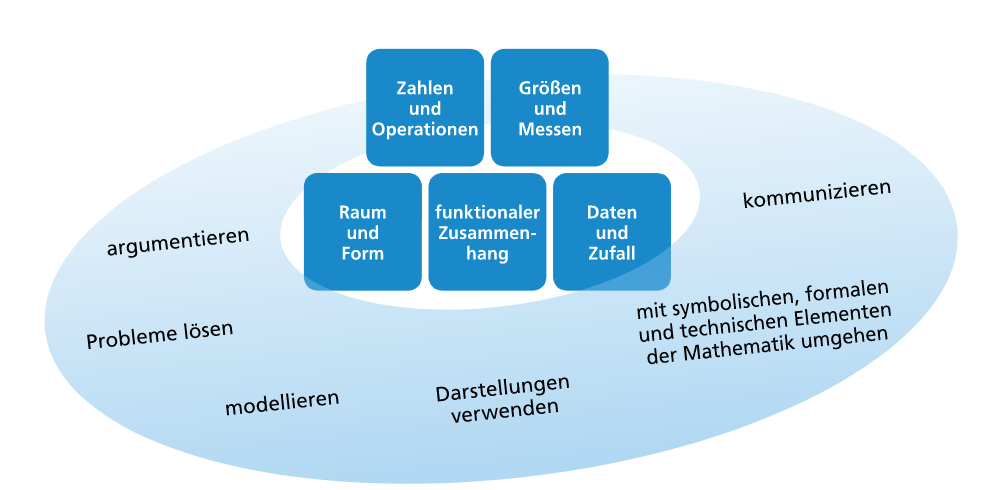
\includegraphics[scale = 0.6]{Kompetenzstrukturmodell.png}\\
\subsection{Beitrag zu übergreifenden Bildungs- und Erziehungszielen}
Das Projekt \glqq Erstellen von Erklärvideos\grqq$~$ bietet vielfältige Möglichkeiten zu den übergreifenden Bildungs- und Erziehungszielen des Lehrplan beizutragen. \\
Die Aufgeschlossenheit des Gymnasium gegenüber neuen Anforderungen im fachlichen wie methodischen Bereich ermöglicht es neue Lernwege, wie das gemeinsame Erstellen von Erklärvideos im Mathematik-Unterricht zu gehen.\\
Diese Methode ermöglicht die gezielte Förderung der geistigen Wendigkeit, eigenständigen Problemlösung, zielgerichteten Zusammenarbeit in der Gruppe und ermöglicht den Schülern das Einnehmen verschiedener Blickwinkel auf die darzustellende Thematik. Letzteres wird von den Schülern allein dadurch gefordert, da sie zwischen der Sichtweise des Produzenten bzw. Rezipienten wechseln. \cite{LehrplanPlusBildungsziele}\\
Das Projekt holt die Schüler direkt aus ihrer Lebenswirklichkeit ab, die inzwischen sehr von medialem Konsum, auch in Form von Erklärvideos \cite{jim16} geprägt ist. Die Schüler setzen neue Medien und Informationstechnologien ein, um den Projektauftrag  zu erfüllen. Dadurch wird die Lernmotivation gefördert und in der Vorbereitungsphase des Projekts \ref{Vorbereitungsphase} die eigenständige Erschließung des Wissens unterstützt. Im Rahmen der Teamsitzungen und Festlegung von Zwischenzielen wird ihnen jederzeit die Möglichkeit eingeräumt ihr Handeln hinsichtlich \glqq Effizienz des individuellen und gruppenorientierten Lernverhaltens\grqq $~$ \cite{LehrplanPlusBildungsziele} zu evaluieren.\\
Die Schüler gestalten den Unterricht in dieser Phase aktiv mit und erleben wie sie selbst zu Lehrenden werden, die fachliche Inhalte mittels Videografie vermitteln. Dies fördert ebenso den Gemeinschaftsgeist der Klasse. Sie lernen sich mit den Vorstellungen anderer auseinanderzusetzen. Eine Fähigkeit die unabdingbar für das Erstellen eines qualitativ hochwertigen Videos ist, da die Schüler nur so beurteilen können, welche Inhalte sie in welcher Tiefe erklären müssen, um dem Zuschauer beim Verständnis der Thematik zu helfen. \\
Das Projekt eröffnet kooperative Arbeitsfelder, die zeigen, dass nicht nur isoliertes Fachwissen, sondern fächerübergreifenden Wissenserwerb zählt. Somit ermöglicht das Projekt fächerübergreifendes Lernen. Betrachtet man das Fachprofil Kunst, so gibt es zahlreiche Überschneidungen im Bereich des Einsatzes von Medienformen und der eigenständigen Entwicklung medialer Inhalte und der ästhetischen Grundbildung. So könnte die Erstellung der Bilder, Zeichnungen und Präsentationen in Zusammenarbeit mit dem Kunstlehrer erfolgen, der die Schüler bezüglich der Komposition und Bildbearbeitung, sowie beim Gestalten der Zeichnungen unterstützt. Vor allem in den Jahrgangsstufen 5 - 8 finden sich Überschneidungen in den Lernbereichen des Faches Kunst mit den Anforderungen an das Erstellen eines Erklärvideos. 
\begin{center}
	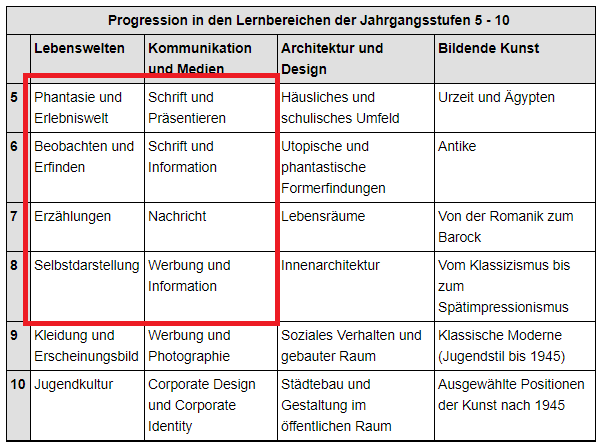
\includegraphics[scale = 0.3]{KunstFachprofil.png} 
\end{center}
Auch das Fach Deutsch ist bietet bei naturgemäß sprach-basierten Erklärvideos viele Anknüpfungspunkte. Der Erfolg des Erklärvideos hängt maßgeblich von dem fähigen Umgang mit Sprache ab. Das Fach Deutsch schult das Sprechen und Kommunizieren, sowie das Schreiben wie es kein anderes Fach vermag. Möglichkeiten der Zusammenarbeit bäten sich vorwiegend im Gebiet der Drehbucherstellung und in der Drehphase des Projekts an, bei der die Schüler bei der rhetorischen Gestaltung ihres Videos vom Deutschlehrer unterstützt werden könnten. Vor und während der Drehbucherstellung beschäftigen die Schüler sich mit der \glqq Recherche, Analyse und Aufbereitung von Informationen\grqq $~$, um zu fachlichen Experten zu werden. Sie erwerben und stärken die Fähigkeit selbstbestimmt, gezielt Informationen zu beschaffen. In diesen Gebieten kann macht eine Zusammenarbeit mit dem Fach Deutsch ebenfalls Sinn.  \\
Abhängig von der gewählten Thematik der Erklärvideos bieten sich Zusammenarbeiten mit vielen weiteren Fächern, wie beispielsweise Physik, Geschichte oder Biologie an. \\ 
Das Projekt schult überfachliche Kompetenzen der Schüler, wie die Selbstkompetenz durch die Rollenzuteilung und Übernahme von Verantwortung im Team sowie das selbstbestimmte Lernen. Da die Schüler in Teams arbeiten und gemeinsam ein Produkt erstellen, mit dem sich jedes Teammitglied identifizieren kann, erwerben und stärken sie die Sozialkompetenz. Nur mithilfe einer konstruktiven Kommunikation im Team und der Mitarbeit jedes Einzelnen gelingt es das gesetzte Ziel zu erreichen. \\
Die Schüler erwerben ebenso Kenntnisse und Fähigkeiten im Bereich der Medien- und technischen Bildung. Die Schüler entwickeln ein Bewusstsein für den Umgang mit Daten aus dem Netz. Sie setzen sich mit den rechtlichen Bestimmungen für die Mediennutzung, wie dem Urheberrecht oder Datenschutz beispielsweise, auseinander. 



\subsubsection{Möglichkeiten der Förderung mathematischer Kompetenzen}
Aber nicht nur die übergreifenden Bildungsziele werden gefördert. Beim Erstellen eines Erklärvideos werden viele mathematische Kompetenzen bedient, die im modernen Mathematikunterricht eine wesentliche Rolle spielen. \\
Im folgenden sollen nur die prozessbezogenen Kompetenzen (hellblaue Ringe) genauer betrachtet werden. \\
\paragraph{Mathematisch Kommunizieren}
Allgemein gilt, dass Projekte in denen Erklärvideos im Mathematikunterricht erstellt werden, unabhängig von der genauen Themenstellung die Kompetenz \glqq Mathematisch Kommunizieren\grqq fördern.  Die Schüler trainieren diese Fähigkeit, da sie Aufgaben und Texte zu mathematischen Inhalten verstehen müssen, bevor sie das Wesentliche zusammenfassen und in eigenen Worten erklären können. Das gemeinsame Arbeiten innerhalb dieser Lernumgebung, die zur Eigenaktivität anregt, erfordert von den Schülern in verschiedenen Phase der Projektarbeit mathematische Kommunikation. \\
Zu Beginn des Projekts steht die Stärkung der passiven Komponente dieser Kompetenz im Vordergrund. Im Prozess der Erarbeitung der fachlichen Inhalte, müssen die Schüler mathematische Aufgabenstellungen und Texte verstehen. Sie kommunizieren auch aktiv mit ihren Teammitgliedern und tauschen sich gegenseitig über die mathematischen Inhalte und den individuellen Wissenserwerb aus. Sobald es an die Erstellung des Drehbuchs rückt die aktive Komponente der Kompetenz K6 in den Vordergrund. Nun beschreiben die Schüler  in eigenen Worten die mathematischen Inhalte und präsentieren diese unter Verwendung der Fachsprache in angemessener Form\\ %Zitieren aus Lehrplan steht da so fast wörtlich
\paragraph{Mathematische Darstellungen verwenden}
Eine weitere Kompetenz, die durch diesen unterrichtlichen Zugang in den Vordergrund rückt, ist die Fähigkeit zur Verwendung mathematischer Darstellung. Unabhängig von dem konkreten mathematischen Thema zu dem die Schüler ein Erklärvideo erstellen, müssen sie ihr Wissen mithilfe von Zeichnungen, Formeln, Skizzen, Fotos oder auch Diagrammen vermitteln, da Erklärvideos auch zu großen Teilen visuell aufgenommen werden. Sie wechseln zwischen verschiedenen Darstellungsformen (Skizze, Formel, reale Situation) und präsentieren die Zusammenhänge in geeigneter Weise. \\
\paragraph{Mathematisch Argumentieren}
Im Diskurs mit den Teammitglieder über die Inhalte des Drehbuchs, die Verknüpfung einzelner Szenen und die gewählten Darstellung symbolischer wie bildlicher Art 
% Einzelne Kompetenzen genauer beschreiben!


\glqq Mathematisch Argumentieren\grqq$~$, \glqq Mathematisch Modellieren\grqq$~$, \glqq Mathematische Darstellungen\grqq$~$ trainieren die Schüler bei der Entwicklung des Drehbuchs und Storyboards.
%Stichpunkt Lernen durch Lehren Förderung mathematischer Kompetenzen modellieren, kommunizieren, argumentieren


\subsection{Erwartungshorizont}
\section{Ablauf des Projekt Erstellung eigener Erklärvideos}
Im Rahmen dieser Arbeit wurden mit einer achten Klasse des Ammerseegymnasiums in Dießen Erklärvideos zum Thema \glqq Abgrenzung des Begriffs Laplace-Experiments\grqq$~$ erstellt. Die Schüler erstellten Videos im Stil der \glqq Legetrick-Technik\grqq $~$, \glqq Screencast-Videos\grqq$~$ und sogenannte \glqq Draw-My-Life-Videos\grqq. Die Schüler arbeiteten in Dreier- bzw. Vierergruppen und erhielten alles das selbe Thema. Auf eine Unterteilung des Themas und Aufteilung der Unterthemen auf die Schüler wurde bewusst verzichtet. Die einzige sinnvolle Aufteilung wäre die Unterteilung in drei große Gruppen, die die Unterthemen: \textcolor{yellow}{Laplace-Experiment}, \textcolor{violet}{Zufallsexperimente, die die Laplace-Annahme zunächst nicht erfüllen durch Verfeinern des Ergebnisraums jedoch entsprechend modelliert werden können} und \textcolor{green}{Zufallsexperimente, die nicht tragfähig als Laplace-Experimente modelliert werden können}. Eine derartige Teilung hätte allerdings dazu geführt, dass bei den beiden letzteren Themen trotzdem sämtliches Wissen über Laplace-Experimente vorausgesetzt wird während die Gruppe, die Erklärvideos über Laplace-Experimente erstellt, das Lernziel des Projekts erst nach dem Anschauen der Videos der anderen beiden Gruppen erreichen kann. 


  
 \subsection{Allgemeines zum Projektablauf}
 Die Erklärvideos wurden mithilfe der beiden von der Schule bereitgestellten Kameras, sowie Laptops und dem Programm Prezi und Screencast-o-matic erstellt. \\
 Das Projekt beginnt mit der Erarbeitung der fachlichen Inhalte. Das Ziel dieser Phase ist, dass die Schüler mithilfe bereitgestellter Materialien sich nötiges Wissen aneignen und zu fachlichen Experten werden. Aufbauend darauf beginnt die Erstellung der Drehbücher, in denen die Schüler ihr Wissen strukturieren und die wichtigsten Aspekte herausarbeiten. Basierend auf den Drehbüchern erstellen die Schüler je nach Videotyp, ein Storyboard oder eine Präsentation. Die Schüler mussten sich im Vorfeld für einen der angebotenen Videotypen entscheiden und erhielten dementsprechende Arbeitsaufträge. Die Videotypen wurden nach technischer Umsetzbarkeit, Eignung für das Thema und unter der Prämisse keine Bildaufnahmen von Schülern zu erstellen, ausgewählt. Die für die Videos benötigten Bilder wurden entweder selbst gezeichnet von den Schülern, selbst fotographiert oder lizenzfreie Bilder verwendet. \\
 Wie unter den rechtlichen Voraussetzungen begründet wurde, verwendeten die Schüler lediglich Schulgeräte (\ref{RechtlicheVoraussetzungen}). Manche Videotypen, wie \glqq Draw-My-Life\grqq $~$ Videos, ziehen einen enormen Schneideaufwand nach sich. Da eine entsprechende Einarbeitung der Schüler zu zeitaufwendig und im Vergleich dazu wenig gewinnbringend gewesen wäre, wurde dies von der Lehrkraft übernommen. \\
 Der Lehrplan sieht für die Behandlung des Themenkomplexes Laplace-Experimente insgesamt 12 Stunden vor. Da das Thema dieser Arbeit lediglich einen Aspekt der Laplace-Experimente zu deren Abgrenzung bedient, sind für dieses Thema drei Schulstunden vorgesehen. Dies hätte für das durchgeführte Projekt nicht ausgereicht. Der Bearbeitungsszeitraum des Themas wurde auf vier Wochen erhöht und so gelegt, dass die Videos ein paar Tage vor der Schulaufgabe fertig gedreht waren. Über einen Onlinekurs auf der Plattform \textit{mebis} konnten die Schüler die fertigen Erklärvideos als Vorbereitung für die Schulaufgabe anschauen. Die zur Verfügung stehende Zeit wurde auf die unterschiedlichen Phasen aufgeteilt, die nachfolgend genauer vorgestellt werden. Nach Abschluss des Projekts fand eine Filmvorführung statt, in der die Schüler die Erklärvideos gegenseitig nach von ihnen festgelegten Kriterien evaluierten. 
 \subsection{Projektplanung}
 Der projektorientierte Zugang zu dem Thema Abgrenzung des Begriffs Laplace-Experiment erfordert im Vorfeld eine ausführliche Planung. Zum einen müssen die zeitlichen Rahmenbedingungen von der Lehrkraft festgelegt werden und alle nötigen Materialien und Medien zur Verfügung gestellt werden. Da das Erstellen eines Erklärvideos, wie im Punkt \ref{RechtlicheVoraussetzungen} bereits erläutert, datenschutzrechtlichen Einschränkungen unterliegt, muss vor Beginn der Dreharbeiten die entsprechende Einverständniserklärung (s. Anhang) unterschrieben und abgegeben worden sei. \\
 Des weiteren mussten die Stative, Kameras, Laptops, und Plakate, die zum Dreh benötigt werden, in der Schule von der Lehrkraft organisiert werden. 
 \subsubsection{Einteilung der Arbeitsgruppen}
 Die Gruppengröße wurde auf 3-4 Schüler festgelegt, da in dieser Größe die vielfältigen Aufgaben arbeitsteilig in der vorgegebenen Zeit erledigt werden können.  Die Schüler durften sich selbstständig in Gruppen dieser Größe zusammenfinden. Dabei mussten die Schüler sich innerhalb der Gruppen Rollen zuteilen. Diese Verteilung von Zuständigkeiten mithilfe sogenannter Rollenkarten hat sich in der Projekttheorie bewährt \ref{VerteilungVerantwortung}. Ein zusätzlicher Vorteil der Rollenkarten war, dass die Schüler sich verpflichtet fühlten ihren entsprechenden Part zum Projekt beizutragen. Die Beispiele, die die Schüler im Erklärvideo zur Abgrenzung des Begriffs \glqq Laplace-Experiment\grqq verwenden, durften sie selbstständig in der Gruppe auswählen. Dabei standen ihnen unterstützend die bereitgestellten Stationen zu verschiedenen Zufallsexperimenten zur Verfügung. 
 Folgende Gruppen haben zusammengearbeitet und sich für den entsprechenden Videotyp und die genannte Szenerie entschieden:
 \begin{longtable}{|p{0.2\textwidth}|l|p{0.3\textwidth}|}\hline
 	\textbf{\large{Schüler 8A}}& \textbf{\large{Videotyp}} & \textbf{\large{Szenerie}}\\\hline
 	Amadeo, Urban, Paul & Screencast-Video mit Prezi & Welt der Würfel\\\hline
 	Josephine, Antonia, Sophie & Screencast-Video mit Prezi & Oktoberfest - Glücksradstand\\\hline
 	Helena, Melina, Sebastian, Noah & Schiebe-Lege-Technik Erklärvideo & Glücksspiele in Schlumpfhausen\\\hline
 	Yannic, Fynn, Fabio, Julius & Erklärvideo im Draw-My-Life-Stil & Drehen eines Glücksrads \\\hline
 	Max, Yannick, Tim & Screencast-Video mit Prezi & Ziehen aus einer Lostrommel, Würfelwurf\\\hline
 	Emilia, Melissa, Elena, Katharina & Schiebe-Lege-Technik Erklär-Video & Jahrmarkt\\\hline 
 	Viktoria, Amelie, Lucas & Screencast-Video mit Prezi & Drehen eines Glücksrads\\\hline
 \end{longtable}
\subsubsection{Organisation der Arbeitsgruppen}
%Hier Erklärung Rollen plus TODO- Plakat (siehe Rauscher Franzi)
 \subsubsection{Projektablaufplan}
Für den Dreh der Videos sollte viel Zeit eingeplant werden. Der Zeitplan sieht folgendermaßen aus:\\
\begin{longtable}{|c|c|p{0.8\linewidth}|}\hline
\cellcolor{yellow}Tag&\cellcolor{violet}Datum & \cellcolor{cyan}Inhalt\\\hline
1&\cellcolor{pink}09.05.2016& Einführung in das Projekt, Vorstellung der Videotypen und entsprechende Beispielvideos, Festlegung der Gruppen und Einteilung der Rollen, Vorstellung des Zeitplans und Portfolios, Auswahl des Videotyps in den Gruppen\\\hline
2&\cellcolor{pink}10.05.2016& Bearbeiten der bereitgestellten Stationen, Erstellung einer Mindmap mit den wichtigsten Begriffen, die im Video vorkommen sollen, Festlegung des Projektauftrags \\\hline
3&\cellcolor{pink}11.05.2016&Erstellen des Drehbuchs \\\hline
4&\cellcolor{pink}12.05.2016&Erstellen des Drehbuchs \newline HA: Finalisieren des Drehbuchs\\\hline

5&\cellcolor{pink}16.05.2016& 1. Teamsitzung - Besprechung und Überarbeitung des Drehbuchs\\\hline
6&\cellcolor{pink}17.05.2016&Erstellung des Zeichnungen bzw. der Präsentation HA: Anfertigen der nötigen Bilder\\\hline
7&\cellcolor{pink}18.05.2016&Erstellung des Zeichnungen bzw. der Präsentation\\\hline
8& \cellcolor{pink}19.05.2016&Finalisierung der Präsentationen \\\hline

9&\cellcolor{pink}23.05.2016& 2. Teamsitzung - Besprechung der Präsentationen und Storyboards,
1. Drehtag - Probedreh\\\hline
10&\cellcolor{pink}24.05.2016& 3. Teamsitzung - Besprechung der Probeaufnahmen, 2. Drehtag\\\hline
\rowcolor{red}11&\cellcolor{pink}25.05.2016&  Stundenausfall Christi Himmelfahrt\\\hline
12&\cellcolor{pink}26.05.2016&\\\hline

13&\cellcolor{pink}23.05.2016& Filmvorführung und Feedback der Schüler zu den einzelnen Erklärvideos\\\hline
\rowcolor{yellow}14&\cellcolor{pink}24.05.2016& Schulaufgabe\\\hline
15&\cellcolor{pink}25.05.2017&Preisverleihung für die von den Schülern zu den besten drei Filmen gewählten Erklärvideos,  Feedback zum Projekt Erstellen von Erklärvideos zum Thema \glqq Laplace-Experiment- Ja, Nein, Vielleicht?\grqq\\\hline
\end{longtable}


\subsection{Realisierungsphase - Durchführung im unterrichtlichen Rahmen}
\subsubsection{Erarbeitung der fachlichen Inhalte} 
Der Einstieg in das Lehrplankapitel \glqq Laplace-Experimente\grqq erfolgte bereits zwei Wochen zuvor mit einer Einführung in die wichtigsten Begriffe bei Zufallsexperimenten, die Erarbeitung der Definition eines Laplace-Experiments und der Formel zur Berechnung von Laplace-Wahrscheinlichkeiten. Den Schülern war aber noch nicht bewusst, dass Zufallsexperimente nicht zwangsläufig Laplace-Experimente sind, und dies oft von der Wahl der Ergebnisraumes abhängt. \\ In der ersten Stunde wurde das Ziel des projektorientierten Zugangs, das Erstellen eines Erklärvideos zum Thema \glqq Laplace-Experiment - Ja, Nein oder Vielleicht?\grqq, vorgestellt. Zwei Beispielvideos, eines von Simple Math %\cite{SimpleMathVideo}
und ein Video, das die Schiebe-Lege-Technik verwendet. Um zu vermeiden, dass die Schüler sich unterbewusst an dem vorgestellten Video orientieren und ihre Kreativität eingeschränkt wird, wurden bewusst zwei Videos ausgewählt, die ihre Formate ansprechend repräsentieren, jedoch nicht die gleichen Inhalte wie du zu erstellenden Erklärvideos behandeln. \\
Im Unterrichtsgespräch erarbeiteten die Schüler die wesentlichen Charakteristika der einzelnen Videotypen. Schnell wurde als wesentliche Anforderung die Knappheit und einfache, humorvolle Sprache bei Screen-Cast-Videos hervorgehoben. Im Bereich der Schiebe-Lege-Technik-Videos stellten die Schüler fest, dass die Inhalte in kleinen Geschichten mit Protagonisten verpackt waren. Die Schüler erkannten die Notwendigkeit ihre wesentlichen Gedankengänge im Rahmen eines Portfolios festzuhalten und ein Drehbuch zu erstellen. Da die Schüler sich bisher nur mit Laplace-Experimenten, nicht aber mit deren Abgrenzung, beschäftigt hatten, lautete die erste Aufgabe an die Teams sich unter Zuhilfenahme der Stationen mit der Thematik vertraut zu machen. Jede Gruppe musste mindestens zwei der bereitgestellten Stationen bearbeiten. Erfahrungsgemäß war zu erwarten, dass die Schüler die Beispiele mit deren Hilfe sie im Video das Laplace-Experiment abgrenzen, inspiriert von den bearbeiteten Stationen auswählen. Deshalb wurden von jeder Station nur je 4 Exemplare zur Verfügung gestellt. So sollte sichergestellt werden, dass nicht jede Gruppe die selben Beispielexperimente wählt und die Videos zu ähnlich werden.\\
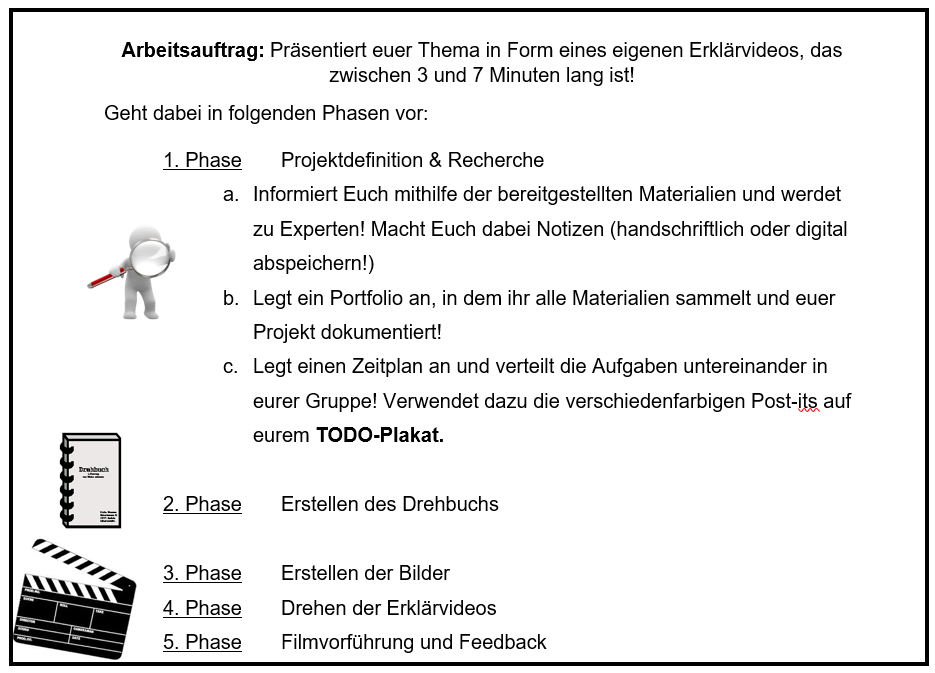
\includegraphics[scale = 0.6]{Projektauftrag.png}\\
Die Stationen setzten sich aus unterschiedlichen Arten von Zufallsexperimenten zusammen. Das Hauptziel der einzelnen Stationen ist jedoch gleich, die Schüler erkennen mithilfe verschiedener Zufallsexperimente, dass nicht jedes Zufallsexperiment ein Laplace-Experiment ist. Sie erarbeiten, dass es von der Ergebnismenge eines Zufallsexperiments abhängt, ob die Laplace-Annahme erfüllt ist. Sie beschreiben außerdem Zufallsexperimente, die nicht als Laplace-Experimente modelliert werden können. Die Schüler begründen mithilfe von Beispielen, dass die Laplace-Wahrscheinlichkeit sich nicht eignet um einen allgemeinen Wahrscheinlichkeitsbegriff zu definieren. \\
\large{\textbf{Stationen zur Erarbeitung der fachlichen Inhalte}}\\
\begin{itemize}
	\item[(a)] Die Station \glqq Welt der Würfel\grqq beschreibt Zufallsexperimente bei denen es um das Werfen eines Würfels geht. Dabei werden verschiedene Würfel betrachtet. Die Schüler erkennen in dieser Station, dass der Würfelwurf nicht automatisch ein Laplace-Experiment ist. Sie beschreiben, dass der Wurf mancher Würfel (z.B. gezinkter Würfel) aufgrund der nicht erfüllten Bedingung der Gleichwahrscheinlichkeit der Ergebnisse, kein Laplace-Experiment ist. Darunter gibt es jedoch Würfel, bei denen die Ergebnismenge bei einem Würfelwurf so verändert werden kann, dass die Gleichwahrscheinlichkeit der Ergebnisse gilt. \\
	Die letzte Aufgabe beschäftigt sich mit dem Spiel \glqq Die Siedler von Catan\grqq. Hier erkennen die Schüler, dass es sich beim zweifachen Würfelwurf bei Betrachtung der Augensumme um kein Laplace-Experiment handelt. Werden jedoch die Werte der einzelnen Würfel unterschieden, kann die Ergebnismenge so verfeinert werden, dass alle Ergebnisse gleich wahrscheinlich sind.  
	\item[(b)] Die Station \glqq Das Glücksrad\grqq betrachtet entsprechende Zufallsexperimente. Je nachdem wie die Sektoren eines Glücksrads gestaltet sind und abhängig von der betrachteten Ergebnismenge handelt es sich um ein Laplace-Experiment oder nicht. Die Schüler erarbeiten, dass sie bisher nur die Wahrscheinlichkeit von Ergebnissen bzw. Ereignissen bei Laplace-Experimenten berechnen können. Diese Erkenntnis führt dazu, dass sie versuchen Zufallsexperimente als Laplace-Experiment zu modellieren durch Angabe einer Ergebnismenge, die die Laplace-Annahme erfüllt. Hierbei hilft ihnen die Unterteilung eines Glücksrads in gleich große Sektoren und deren Nummerierung. Die letzte Aufgabe soll bei Schülern die Einsicht wecken, dass die Laplace-Wahrscheinlichkeit sich nicht als allgemeine Wahrscheinlichkeitsdefinition eignet. 
	\item[(c)] Die Station\glqq Verrückte Kartenwelt \grqq beschreibt Zufallsexperimente, bei denen es um das Ziehen aus einem Kartenstapel geht. Dabei sind die Kartendecks unterschiedlich zusammengesetzt. Die Schüler beurteilen wann es sich um ein Laplace-Experiment handelt und geben die entsprechenden Ergebnismengen an. 
	\item[(d)] Die Station \glqq Lose, Lose, Lose\grqq$~$ liefert den Schülern Anreize für Zufallsexperimente, die auf Urnen-Experimenten beruhen. Im Vergleich mit einer vereinfachten Version des Roulettespiels erkennen die Schüler, dass sie die Wahrscheinlichkeiten gewisser Ereignisse nur berechnen können, wenn sie die Zufallsexperimente als Laplace-Experimente modellieren.  
\end{itemize}
Die Ergebnisse der Stationenarbeit fassen die Schüler im Portfolio zusammen. Im Team ist in dieser Phase die Rolle des \glqq Mathe-Cracks\grqq Die Lehrkraft fungiert in dieser Phase in einer beratenden Rolle. Sie unterstützt die Schüler bei der fachlichen Erarbeitung und stellt zur Überprüfung Lösungsvorschläge zu den einzelnen Stationen bereit.
\subsubsection{Erstellen des Drehbuchs - Unterteilung und Festlegung von Schwerpunkten}$~$\newline
Die Schüler agieren nun als fachliche Experten. Sie besitzen einen Überblick über das Thema und sind in der Lage die essentiellen Elemente herauszuarbeiten. Dies geschieht während der Erstellung des Drehbuchs. Nun legen die Schüler im Projektauftrag ihre genaue Zielbeschreibung des Erklärvideos fest und entwickeln auf ihrem Wissen basierend die elementaren Szenen des Videos. Bevor die Schüler die Texte verfassen, entscheiden sie im Team, welche Zufallsexperimente im Video betrachtet werden sollen. Diese Entscheidung hängt natürlich ebenfalls davon ab in welcher Szenerie die Videos spielen. Diejenigen Gruppen, die die Legetrick-Technik verwenden, müssen darauf achten, dass die gewählten Zufallsexperimente sich in einer Geschichte verbinden lassen. Hierfür ist besonders die Rolle des \glqq Creative Directors\grqq$~$ verantwortlich. 
\subsubsection{Erstellen der Bilder/Präsentation}
\subsubsection{Drehen der Videos}
\subsection{Präsentation der Erklärvideos}
\subsection{Beurteilungsphase}
\section{Evaluation}
\subsection{Allgemeines zur Evaluation}
\subsection{Evaluation des Kompetenzerwerbs}
\subsection{Chancen und Grenzen des Projekts}
\section{Schluss}
\newpage
\section{Literaturnachweise}
\nocite{lp17}\nocite{jim16}\nocite{daten}
\bibliography{literaturverzeichnis}
\bibliographystyle{alphadin}
\newpage
\section{Eigenständigkeitserklärung}
Ich versichere hiermit,dass ich die vorliegende schriftliche Hausarbeit in allen Teilen selbsständig angefertigt und keine anderen als die angegebenen Hilfsmittel benutzt habe. Alle Stellen, die wörtlich oder sinngemäß aus veröffentlichten oder nicht veröffentlichten Schriften entnommen wurden, sind als solche kenntlich gemacht. Die Arbeit hat in gleicher oder ähnlicher Form noch keiner anderen Prüfungsbehörde vorgelegen. \\\\
Nürnberg, 05.08.2017\\\\
\vspace{0.6cm}\\
$\underline{~~~~~~~~~~~~~~~~~~~~~~~~~~~~~~~~~~~~~~~~~~~~~~~~~~~~~~~~~~~~~~}$\\
\small{Julia Kronawitter, StRefin}
\section{Anlagen}
\subsection{Datenschutzerklärung}
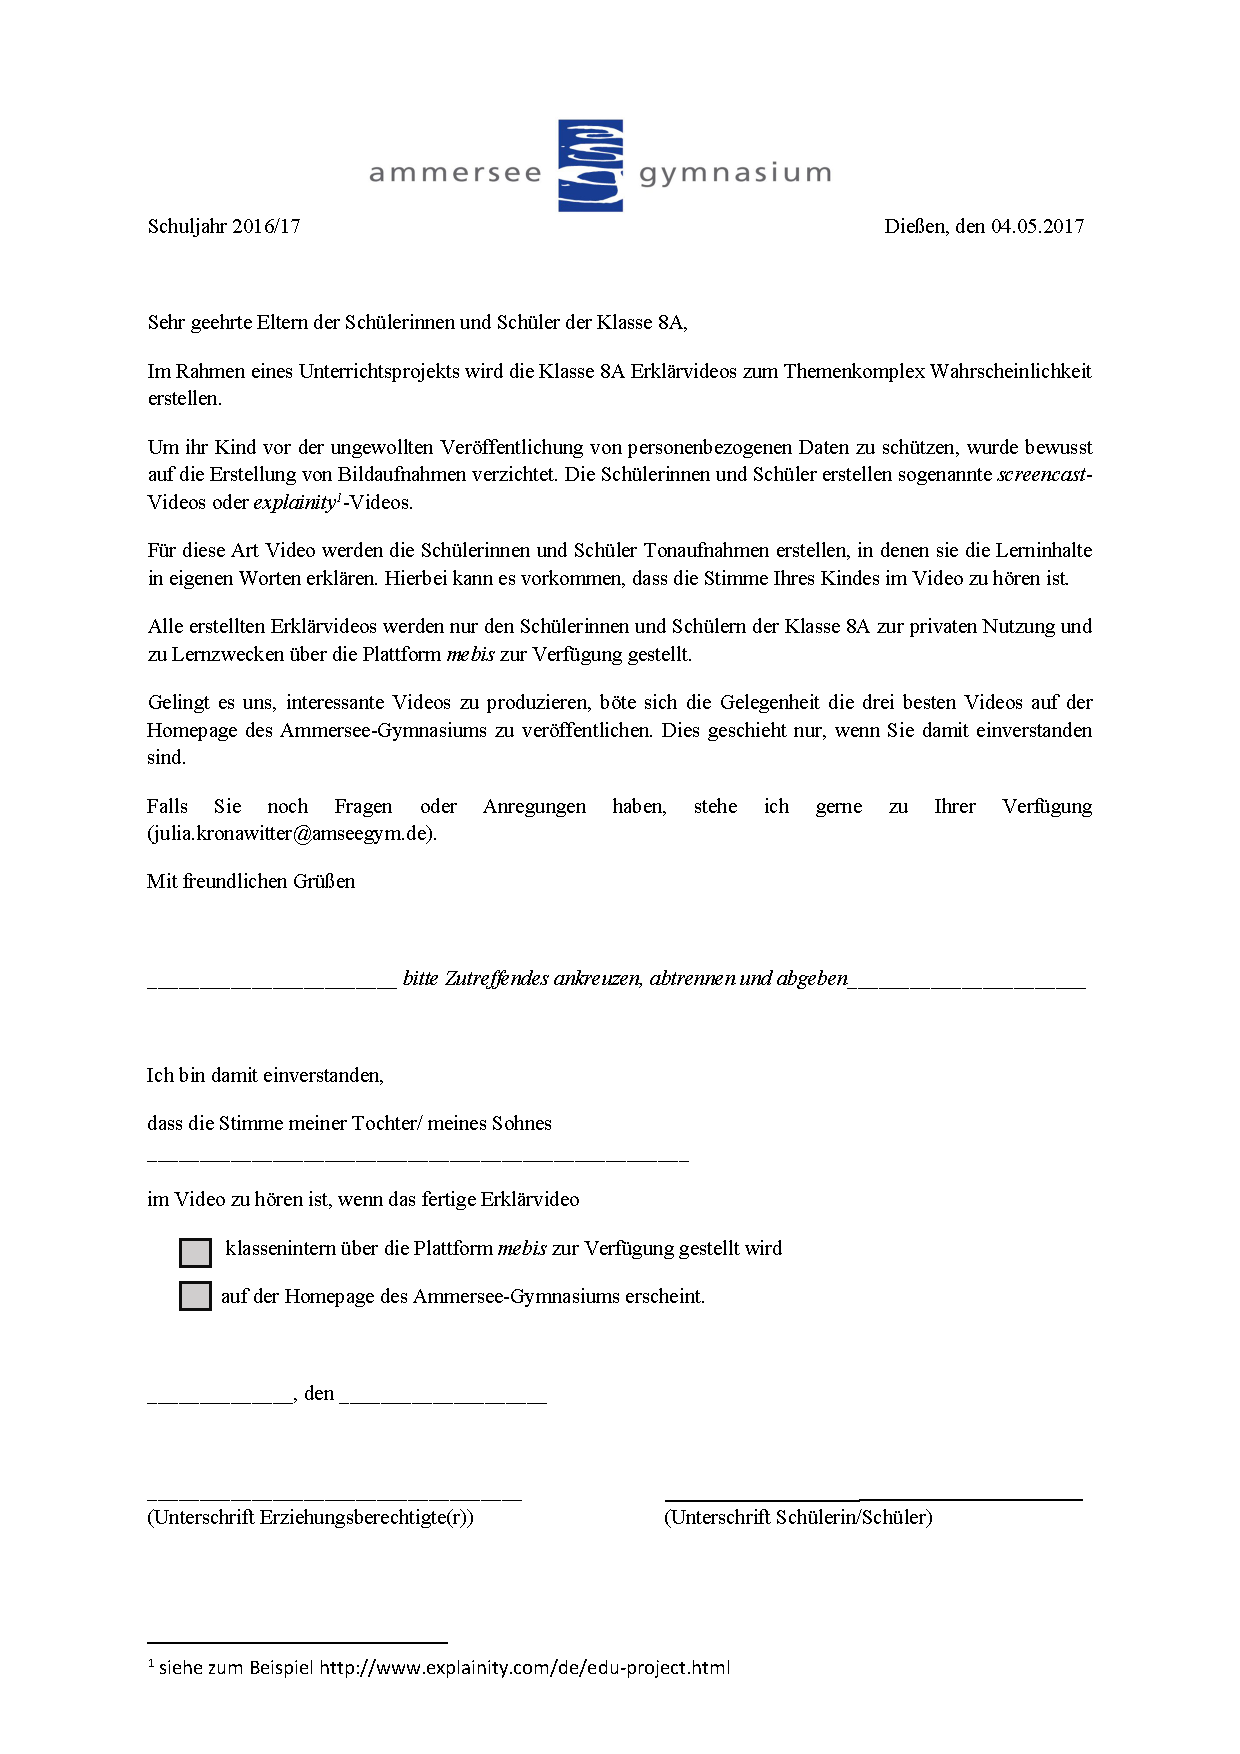
\includepdf{Elternbrief_Bildveroeffentlichung_Version2.pdf}
\subsection{Materalien zur Erarbeitung der Thematik}
\subsection{Arbeitsaufträge}
\subsection{Exemplarische Portfoliomappe zum Thema \glqq Abgrenzung des Begriffs Laplace-Experiment}
\subsection{Evaluationsbogen}
\subsection{Auswertung der Evaluation}

\end{document}